%%%%%%%%%%%%%%%%%%%%%%%%%%%%%%%%%%%%%%%%%%%%%%%%%%%%%%%%%%%%%%%%%%%%%%%%
\documentclass[ms]{osudissert96}
%% Language %%%%%%%%%%%%%%%%%%%%%%%%%%%%%%%%%%%%%%%%%%%%%%%%%
\usepackage[USenglish]{babel} %francais, polish, spanish, ...
%\usepackage[T1]{fontenc}
\usepackage[ansinew]{inputenc}
\usepackage{lmodern} %Type1-font for non-english texts and characters
%% Packages for Graphics & Figures %%%%%%%%%%%%%%%%%%%%%%%%%%
\usepackage{graphicx} %%For loading graphic files
\usepackage[hang]{subfigure}
%% Math Packages %%%%%%%%%%%%%%%%%LAILA%%%%f%%%%%%%%%%%%%%%%%%%%%%%
\usepackage{hyperref}
\setcounter{secnumdepth}{3}
\usepackage{enumerate}
\usepackage{amssymb}
\usepackage{textcomp}
\usepackage{graphicx}
\usepackage{siunitx}
\usepackage{graphics}
\usepackage{epsfig}
\usepackage{epstopdf}
\usepackage{float}
\usepackage{color}
\usepackage[cmex10]{amsmath}
\usepackage{latexsym,amsfonts}
\usepackage{amsthm,bbm}
\usepackage{url}
\usepackage{longtable}
\usepackage[figuresright]{rotating}
\usepackage{listings}
\usepackage{etoolbox}
\usepackage{amsmath}
\usepackage{subfigure}
\usepackage{fancyhdr}   
\usepackage{subcaption}
\pagestyle{fancy} 
\fancyhead{} \fancyfoot{} 
\fancyhead[CO,CE]{\thepage}   
 \usepackage[table,xcdraw]{xcolor}
 
%%%%%%%%%%%%%%%%%%%%%%%%%%%%%%%
\usepackage{amsmath}
\usepackage{amsthm}
\usepackage{amsfonts}
\usepackage{amssymb,amscd,mathrsfs}
\usepackage{epsfig}
\usepackage{longtable}
\usepackage[numbers,sort]{natbib}
%\usepackage[withbib,all]{authorindex}
%\usepackage{esint}
\usepackage{epstopdf}
\usepackage{paralist}
\usepackage{algorithmic}
\usepackage{multirow}
\usepackage{subcaption}
\usepackage[linesnumbered,ruled,vlined]{algorithm2e}
\usepackage{bm}
\newcommand{\vect}[1]{\boldsymbol{\mathbf{#1}}}
\usepackage{epsf,color}
\usepackage{caption}
\usepackage[a4paper,left=15mm,right=15mm, top=1cm, bottom=2cm]{geometry}
\usepackage{tabularx}
\usepackage[export]{adjustbox}
\usepackage[table]{xcolor}
\usepackage[section]{placeins}


\captionsetup[figure]{font=small,skip=1pt}
\newtheorem{theorem}{Theorem}
\newtheorem{lemma}{Lemma}
\newtheorem{definition}{Definition}
\newcommand{\Us}{\mathcal{U}_s}
\newcommand{\Ls}{\mathcal{L}_s}
\newcommand{\Os}{\mathcal{O}_s}
\newcommand{\Op}{\mathcal{O}_p}
\newcommand{\Oq}{\mathcal{O}_q}
\newcommand{\mpd}{\mathrm{MPD}}
\newcommand{\msd}{\mathrm{MSD}}
\newtheorem{proposition}{Proposition}\newtheorem{corollary}[theorem]{Corollary}
\newcommand{\prob}{\mathbb{P}}
\newcommand{\cbs}{C_{B}}
\newcommand{\crs}{C_{R}}
\newcommand{\ct}{C_{\textsl{Total}}}
\newcommand{\pgbs}{\prob (g_{B}(l)=g_{\mathrm{B}})  }
\newcommand{\phbs}{\prob (g_{B}(l)=h_{\mathrm{B}})  }
\newcommand{\pgbsP}{\prob (g_{B}(t)=g_{\mathrm{B}})  }
\newcommand{\phbsP}{\prob (g_{B}(l)=h_{\mathrm{B}})  }
\newcommand{\pgrs}{\prob (g_{R}(l)=g_{\mathrm{R}}) }
\newcommand{\phrs}{\prob (g_{R}(l)=h_{\mathrm{R}}) }
\newcommand{\pgrsP}{\prob (g_{R}(t)=g_{\mathrm{R}}) }
\newcommand{\phrsP}{\prob (g_{R}(l)=h_{\mathrm{R}}) }
\newcommand{\pf}{\prob (r(l)=r) }
\newcommand{\pw}{\prob (r(l)=r) }
\newcommand{\pfP}{\prob (r(t)=r) }
\newcommand{\pwP}{\prob (r(l)=r) }
\DeclareMathOperator{\Exp}{\mathbb{E}}
%%%%%%%%%%%%%%%%%%%%%%%%%%%%%%%%%%%%%%%%%%%%%%%%%%%%%%%%%%%%%
%% DOCUMENT
%%%%%%%%%%%%%%%%%%%%%%%%%%%%%%%%%%%%%%%%%%%%%%%%%%%%%%%%%%%%%
\begin{document}

\author{Author Name}
%% Be sure to use modified style that makes this uppercase
\title{Thesis Name}
\authordegrees{Degree. Ex: B.Sc.}
\graduationyear{2020}
\maketitle
\pagestyle{empty} %No headings for the first pages.

% \startsinglespace
\begin{center}
CERTIFICATION OF APPROVAL
\vskip 30pt
Thesis Title
\end{center}
\vskip 50pt

\makebox[5in][c]{\leaders\hrule\hskip 5in}

Doctor-Name (Committee Chair, Internal Committee Member)

Professor, Nile University
\vskip 20pt

\makebox[5in][c]{\leaders\hrule\hskip 5in}

Doctor-Name (Supervisor)

Associate Professor, Nile University
\vskip 20pt

\makebox[5in][c]{\leaders\hrule\hskip 5in}

TBD (External Committee Member)

Associate Professor, X University
\vskip 20pt

\makebox[5in][c]{\leaders\hrule\hskip 5in}

Doctor-Name (Supervisor)

Assistant Professor, Nile University
\vskip 20pt


\begin{center}
June, 2020
\vskip 10pt
Nile University
\end{center} 

% Copyright the dissertation
\disscopyright
\pagebreak


\startdoublespace
% The abstract
\begin{abstract}
Abstract goes here ...
\end{abstract}
\dedication{To my beloved family}

\acknowledgements{ACKNOWLEDGMENTS goes here ...}


%% Title Page %%%%%%%%%%%%%%%%%%%%%%%%%%%%%%%%%%%%%%%%%%%%%%%
%% ==> Write your text here or include other files.

%\input{title_page}

%% Inhaltsverzeichnis %%%%%%%%%%%%%%%%%%%%%%%%%%%%%%%%%%%%%%%
\tableofcontents %Table of contents
\listoftables
\listoffigures

\cleardoublepage %The first chapter should start on an odd page.

\pagestyle{plain} %Now display headings: headings / fancy / ...

% Include the chapters of the thesis, as separate files
% Just uncomment the lines as you write the chapters

%%%%%%%%%%%%%%%%LIST OF ABBREVIATIONS%%%%%%%%%%%%%%%%%%%%%%%%%%%%%%
\begin{center}
  \textbf{{LIST OF ABBREVIATIONS}}
\end{center}
\begin{longtable}{@{\extracolsep{\fill}}ll@{}}

\centering
\begin{tabular}{l l}
\hline
\textbf{Symbol} & \textbf{Definition} \\
\hline \hline
cDBG & Combact de bruign graph \\
DAG & Directed asyclic graph \\
GTF & Gene transfer format \\

\hline
\end{tabular}
\end{longtable}
% \newpage
% %%%%%%%%%LIST OF SYMBOLS%%%%%%%%%%%%%5
% \begin{center}
%   \textbf{{LIST OF SYMBOLS}}
% \end{center}
% \begin{longtable}{@{\extracolsep{\fill}}ll@{}}

% %\begin{tabular}{l l}
% \hline
% \textbf{Symbol} & \textbf{Definition} \\
% \hline \hline
% $\mathcal{I}$ & Interference power\\
% $\mathcal{N}_o$ & Noise power \\
% $\mathcal{S}$ & Desired signal power \\
% $\alpha$ & Path-loss exponent \\
% $\gamma$ & Signal-to-interference ratio \\
% $\mathcal{L}_X(\cdot)$ & The Laplace transform of the {PDF} of the random variable X  \\ 
% $\vartheta$ & The skewness of the zipf distribution \\
% $R_{SBS}$ & Ergodic Capacity per SBS \\
% $\Gamma(\cdot)$ & The gamma function \\
%  ${_2}F_1(\cdot,\cdot;\cdot;\cdot)$ & Gauss hypergeometric function \\
% $p$ & Independent activity probability \\
% $f_{X}\left( x\right)$ & PDF of random variable X\\
% $F_{X}\left( x\right)$ & CDF of random variable X\\
% $\left\|.\right\|$ & Euclidean norm \\
% $\forall$ & for all  \\
% $\mathbb{E}\left[.\right]$ & The expected value of a random variable \\ 
% $\phi_{u}$ & Set of users in a PPP distributed network \\
% $\phi_{b}$ & Set of SBSs in a PPP distributed network \\
% $\lambda_{u}$ & user intensity in PPP distributed network\\
% $\lambda_{b}$ & SBS intensity in PPP distributed network\\
% $\phi_{p}$ & Parent points set in clustered network \\
% $\lambda_{p}$ & Parent points intensity in clustered network \\
% $\phi_{u_{c}}$ & Set of per cluster users \\
% $\lambda_{u_{c}}$ & Per cluster user intensity \\
% $\phi_{s_{c}}$ & Set of per cluster SBSs \\
% $\lambda_{s_{c}}$ & Per cluster SBS intensity \\
% $I_{o}(.)$ & Modified Bessel function of first order zero kind \\
% $P(m)$ & Probability that file $m$ is requested \\
% $N_{f}$ & Number of files in the network \\
% $N_{c}$ & Cache capacity \\
% $F$ & File Size \\
% $P_{m,j}$ & Probability that the $m^{\rm th}$ file cached in the $j^{\rm th}$ memory location \\
% $\omega_{ca}$ & The caching power consumption \\
% $P_{r, \rm min}$ & Minimum received power \\
% $\omega_{bh}$ & Core network energy consumption \\
% $\delta$ & Outage threshold \\
% $P_{\rm links}$  &  Links power density \\ 
% $P_{\rm nodes}$ & Nodes power density \\ 
% $|.|$ & Cardinality of a Set \\
% \hline

% %\end{tabular}
% \end{longtable}


%%%%%%%%%%%%%%5

% \Huge{\textbf{TEMPORARY OFF - TRANSFORMING THE THESIS STRUCTURE ...}}

\chapter{Introduction}

\section{Motivation}

In figure \ref{chapter1} Lorem Ipsum is simply dummy text of the printing and typesetting industry. Lorem Ipsum has been the industry's standard dummy text ever since the 1500s, when an unknown printer took a galley of type and scrambled it to make a type specimen book. It has survived not only five centuries, but also the leap into electronic typesetting, remaining essentially unchanged. It was popularised in the 1960s with the release of Letraset sheets containing Lorem Ipsum passages, and more recently with desktop publishing software like Aldus PageMaker including versions of Lorem Ipsum.

\begin{figure}[!ht]
    \centering
	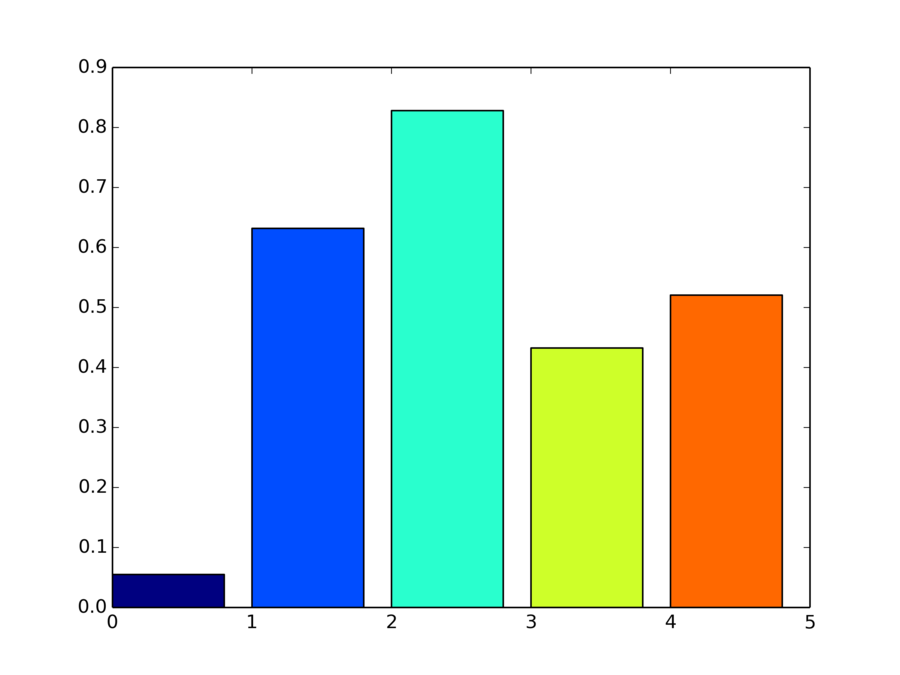
\includegraphics[height=10cm, keepaspectratio]{media/ch1/ch1-1.png}
	\vspace{3pt}
	\caption{Chapter 1 figure 1 caption}
	\label{chapter1}
\end{figure}

\section{Problem Statement}
Lorem Ipsum is simply dummy text of the printing and typesetting industry. Lorem Ipsum has been the industry's standard dummy text ever since the 1500s, when an unknown printer took a galley of type and scrambled it to make a type specimen book. It has survived not only five centuries, but also the leap into electronic typesetting, remaining essentially unchanged. It was popularised in the 1960s with the release of Letraset sheets containing Lorem Ipsum passages, and more recently with desktop publishing software like Aldus PageMaker including versions of Lorem Ipsum.

\section{Thesis Outline and Summary of Contributions}

Lorem Ipsum is simply dummy text of the printing and typesetting industry. Lorem Ipsum has been the industry's standard dummy text ever since the 1500s, when an unknown printer took a galley of type and scrambled it to make a type specimen book. It has survived not only five centuries, but also the leap into electronic typesetting, remaining essentially unchanged. It was popularised in the 1960s with the release of Letraset sheets containing Lorem Ipsum passages, and more recently with desktop publishing software like Aldus PageMaker including versions of Lorem Ipsum.
\chapter{Literature Survey}

\label{Literature Review}

\section{Introduction}

Lorem Ipsum is simply dummy text of the printing and typesetting industry. Lorem Ipsum has been the industry's standard dummy text ever since the 1500s, when an unknown printer took a galley of type and scrambled it to make a type specimen book. It has survived not only five centuries, but also the leap into electronic typesetting, remaining essentially unchanged. It was popularised in the 1960s with the release of Letraset sheets containing Lorem Ipsum passages, and more recently with desktop publishing software like Aldus PageMaker including versions of Lorem Ipsum. \cite{Steinegger2019}.

Lorem Ipsum is simply dummy text of the printing and typesetting industry. Lorem Ipsum has been the industry's standard dummy text ever since the 1500s, when an unknown printer took a galley of type and scrambled it to make a type specimen book. It has survived not only five centuries, but also the leap into electronic typesetting, remaining essentially unchanged. It was popularised in the 1960s with the release of Letraset sheets containing Lorem Ipsum passages, and more recently with desktop publishing software like Aldus PageMaker including versions of Lorem Ipsum.

\section{Section 1}
Lorem Ipsum is simply dummy text of the printing and typesetting industry. Lorem Ipsum has been the industry's standard dummy text ever since the 1500s, when an unknown printer took a galley of type and scrambled it to make a type specimen book. It has survived not only five centuries, but also the leap into electronic typesetting, remaining essentially unchanged. It was popularised in the 1960s with the release of Letraset sheets containing Lorem Ipsum passages, and more recently with desktop publishing software like Aldus PageMaker including versions of Lorem Ipsum.

\subsection{Sub-Section 1}
Lorem Ipsum is simply dummy text of the printing and typesetting industry. Lorem Ipsum has been the industry's standard dummy text ever since the 1500s, when an unknown printer took a galley of type and scrambled it to make a type specimen book. It has survived not only five centuries, but also the leap into electronic typesetting, remaining essentially unchanged. It was popularised in the 1960s with the release of Letraset sheets containing Lorem Ipsum passages, and more recently with desktop publishing software like Aldus PageMaker including versions of Lorem Ipsum.

\subsubsection{Sub-Sub-Section 1}
\textbf{Lorem Ipsum}\hspace{4pt} is simply dummy text of the printing and typesetting industry. Lorem Ipsum has been the industry's standard dummy text ever since the 1500s, when an unknown printer took a galley of type and scrambled it to make a type specimen book. It has survived not only five centuries, but also the leap into electronic typesetting, remaining essentially unchanged. It was popularised in the 1960s with the release of Letraset sheets containing Lorem Ipsum passages, and more recently with desktop publishing software like Aldus PageMaker including versions of Lorem Ipsum.

\chapter{Methodology}

Lorem Ipsum is simply dummy text of the printing and typesetting industry. Lorem Ipsum has been the industry's standard dummy text ever since the 1500s, when an unknown printer took a galley of type and scrambled it to make a type specimen book. It has survived not only five centuries, but also the leap into electronic typesetting, remaining essentially unchanged. It was popularised in the 1960s with the release of Letraset sheets containing Lorem Ipsum passages, and more recently with desktop publishing software like Aldus PageMaker including versions of Lorem Ipsum.
\chapter{Results and Discussions}

\section{Section}

\subsection{Subsection}
\subsubsection{Sub Sub section}

In table \ref{table_1} Lorem Ipsum is simply dummy text of the printing and typesetting industry. Lorem Ipsum has been the industry's standard dummy text ever since the 1500s, when an unknown printer took a galley of type and scrambled it to make a type specimen book. It has survived not only five centuries, but also the leap into electronic typesetting, remaining essentially unchanged. It was popularised in the 1960s with the release of Letraset sheets containing Lorem Ipsum passages, and more recently with desktop publishing software like Aldus PageMaker including versions of Lorem Ipsum.


\begin{table}[]
\begin{tabular}{|c|c|c|}
\hline
\textbf{Col 1}            & \textbf{Col 2} & \textbf{Col 3}            \\ \hline
\cellcolor[HTML]{C0C0C0}1 & 2              & \cellcolor[HTML]{FD6864}3 \\ \hline
1                         & 1              & 2                         \\ \hline
\end{tabular}
\caption{Table one caption}
\label{table_1}
\end{table}


\chapter{Conclusions and Future work}

\section{Conclusion}

Lorem Ipsum is simply dummy text of the printing and typesetting industry. Lorem Ipsum has been the industry's standard dummy text ever since the 1500s, when an unknown printer took a galley of type and scrambled it to make a type specimen book. It has survived not only five centuries, but also the leap into electronic typesetting, remaining essentially unchanged. It was popularised in the 1960s with the release of Letraset sheets containing Lorem Ipsum passages, and more recently with desktop publishing software like Aldus PageMaker including versions of Lorem Ipsum.

\section{Future directions}

Lorem Ipsum is simply dummy text of the printing and typesetting industry. Lorem Ipsum has been the industry's standard dummy text ever since the 1500s, when an unknown printer took a galley of type and scrambled it to make a type specimen book. It has survived not only five centuries, but also the leap into electronic typesetting, remaining essentially unchanged. It was popularised in the 1960s with the release of Letraset sheets containing Lorem Ipsum passages, and more recently with desktop publishing software like Aldus PageMaker including versions of Lorem Ipsum.


%% ----------------------------------------------------------------
% Now begin the Appendices, including them as separate files

\addtocontents{toc}{\vspace{2em}} % Add a gap in the Contents, for aesthetics

% \appendix % Cue to tell LaTeX that the following 'chapters' are Appendices

\chapter{Proof of equation~}

Appendix A goes here...
	% Appendix Title

\chapter{Appendix B Title}

Lorem Ipsum is simply dummy text of the printing and typesetting industry. Lorem Ipsum has been the industry's standard dummy text ever since the 1500s, when an unknown printer took a galley of type and scrambled it to make a type specimen book. It has survived not only five centuries, but also the leap into electronic typesetting, remaining essentially unchanged. It was popularised in the 1960s with the release of Letraset sheets containing Lorem Ipsum passages, and more recently with desktop publishing software like Aldus PageMaker including versions of Lorem Ipsum.
 % Appendix Title



\addtocontents{toc}{\vspace{2em}}  % Add a gap in the Contents, for aesthetics
%\backmatter

%% ----------------------------------------------------------------
\label{Bibliography}
%\lhead{\emph{Bibliography}}  % Change the left side page header to "Bibliography"
\bibliographystyle{IEEEtran}  % Use the "unsrtnat" BibTeX style for formatting the Bibliography
\bibliography{Bibliography}  % The references (bibliography) information are stored in the file named "Bibliography.bib"

\addcontentsline{toc}{chapter}{Bibliography}%

\include{Reference}

\end{document}  % The End
%% ----------------------------------------------------------------